\chapter{Sentence Manager}\label{chap:sentmanager}

The creation of this tool is a consequence of Sentence Reader. When operations upon sentences grow complex, a suitable tool is inevitably needed. Together with Sentence Reader, this tool has cost several months of development, as well as headaches. The Manager is the most complex tool of all, in terms of its functions and components. I cannot tell and show you everything here. I will explain only the basic ideas that you should know when you explore the tool by yourselves. 

Before you read on this chapter, you must understand how the Reader works (see Chapter \ref{chap:sentreader}), and know what I mean by \emph{sentence, sequence, hash, edit,} and \emph{variant}.

Sentence Manager can be launched by menu Sentence > {\faSix \symbol{"F0B1}} Sentence Manager. It can also be opened in the Reader with {\faSix \symbol{"F0B1}} button. Once you have saved a number of sentences and sequences, when you open the Manager, you will see something like Figure \ref{fig:sentmanager-sentences}.

\begin{figure}[!hbt]
\centering
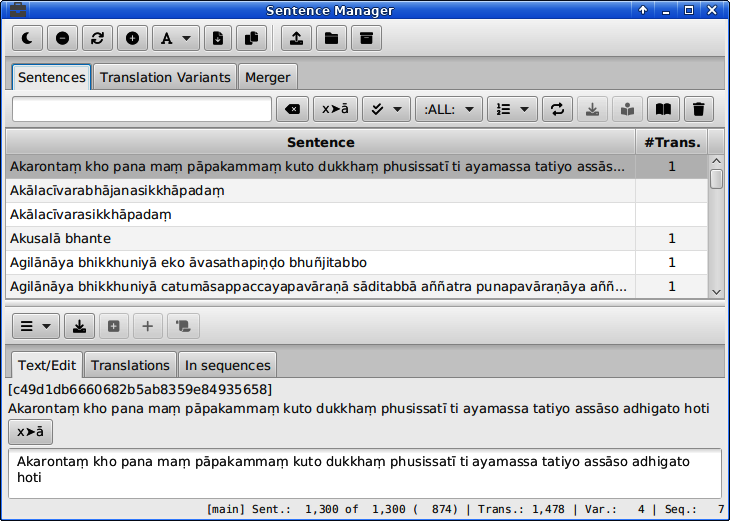
\includegraphics[width=0.9\linewidth]{images/sentmanager-sentences.png}\\
\caption{Sentences in Sentence Manager}
\label{fig:sentmanager-sentences}
\end{figure}

There are three main tabs in the Manager: Sentences, Translation Variants, and Merger. The first two tabs work for one directory at a time. This means there must be at least one working directory. The default is `\texttt{main}'.\footnote{By default, artifacts created by the Reader and Manager are saved in directory \texttt{data/sentences}, but you certainly can use other base directory.} You can change the working directory by {\faSix \symbol{"F07B}} button. Typically, one directory contains many sentence files, several sequence files, and one variant info file.\footnote{In the implementation, sentence and info files are in JSON format. Sequence files are just plain text with \texttt{.seq} extension.}

\section{Sentences}

When the Manager opens a directory, it reads all sentences and lists them in the table, showing the number of translations of each sentence, if any. When some sentences are changed outside the Manager, edited by the Reader, for example, {\faSix \symbol{"F093}} button has to be pressed to update the sentence list. You can save the whole directory into a zip file by hitting {\faSix \symbol{"F187}} button.

On the status bar, the directory's summary is shown. This tells us the directory's name, the sequence's name (if selected), the number of sentences, translations, variants, and sequences. The number in the parentheses is the count of sentences that have translations. When a sequence is selected, the number of the selected sentence is also shown.

In the first open, sentences in the working directory shown in the table are sorted by their text. If the directory has sequences, you can choose to display only a sequence at a time with {\faSix \symbol{"F0CB}} menu button. Once a sequence is selected, the order of sentences in the table will correspond to the order of the sequence. Figure \ref{fig:sentmanager-sequences} shows an example of this selection. Note that `\texttt{:NONE:}' in the menu means `no filtering,' the start-up mode that all sentences are listed and ordered by their text. 

\begin{figure}[!hbt]
\centering
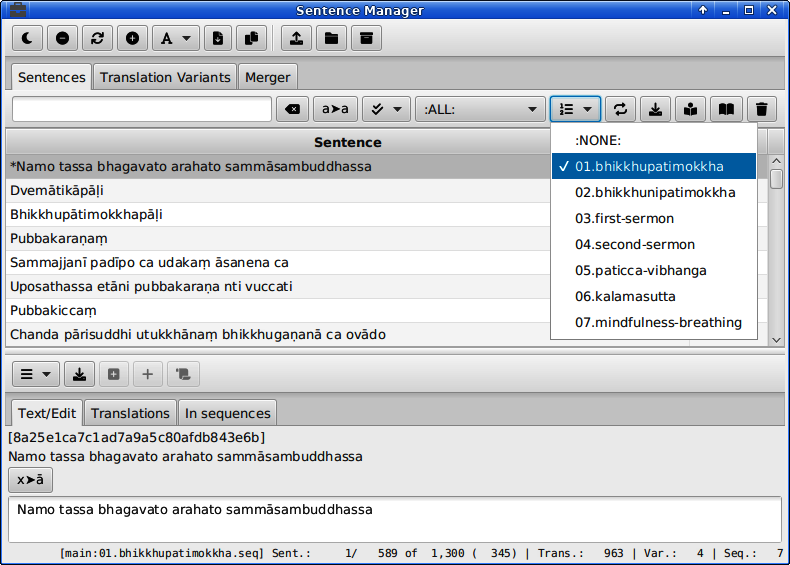
\includegraphics[width=0.9\linewidth]{images/sentmanager-sequences.png}\\
\caption{Selecion of a sequence}
\label{fig:sentmanager-sequences}
\end{figure}

However, the sentence table can also be sorted by its columns. You just click the table headers. When trying this a couple of times, you will see that the order has been changed circularly. One use case of this is when you want to know which sentences have translations more than one. You sort the table by column \emph{\#Trans} and see the rows with greater-than-one translations.

Once you select a sentence, you can edit its text (only the \emph{edit} form is mutable), as well as translations, in the lower part of the window. There are two tabs for the editing purposes. The last tab (\emph{In sequences}) shows the selected sentence across sequences in the working directory. The numbers are the counts of the occurrences if the sentence appears in a sequence. If several sequences have a non-zero number, it shows that the sentence is reused in several places (see Figure \ref{fig:sentmanager-inseq}).

The sentences with an asterisk (*) are those have repeated occurrences in one sequence. Sentences only used across sequences are not marked with the asterisk. Study the counts explained above carefully if you are still curious.

\begin{figure}[!hbt]
\centering
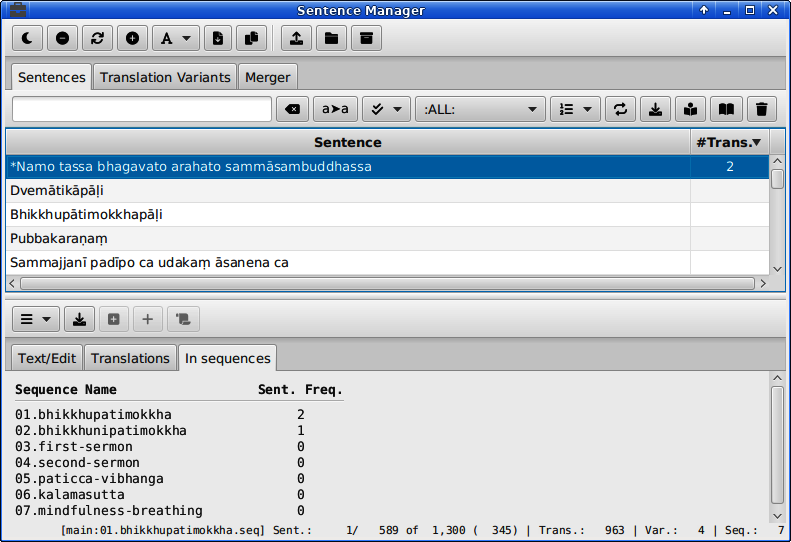
\includegraphics[width=0.9\linewidth]{images/sentmanager-inseq.png}\\
\caption{Statistics of sentence's reuse in sequences}
\label{fig:sentmanager-inseq}
\end{figure}

If you play more attention to translations and want to see sentences having only a particular variant, you can use the dropdown option provided (see Figure \ref{fig:sentmanager-translations}). In the example, I filter only sentences that have translations by Thanissaro (Ven.\,Ṭhānissaro). In the menu, `\texttt{:ALL:}' means all sentences regardless of translations; `\texttt{:ONLY:}' means only the sequence selected as mentioned above; and `\texttt{:NONE:}' means sentences without translations.

\begin{figure}[!hbt]
\centering
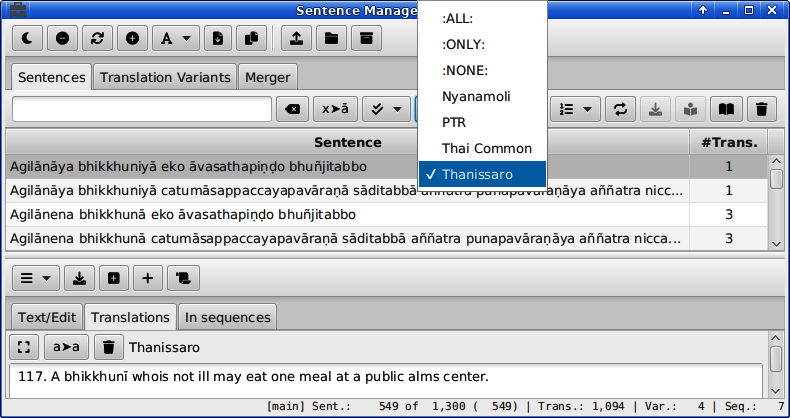
\includegraphics[width=0.9\linewidth]{images/sentmanager-translations.png}\\
\caption{Filtering by translations}
\label{fig:sentmanager-translations}
\end{figure}

You can search for sentences by three options: in (original) text, in edit, and in translations (see {\faSix \symbol{"F560}} button). You can open the selected sequence in a new Sentence Reader by pressing {\faSix \symbol{"F5DA}} button. If you focus only one sentence, you can open it in a new Reader likewise by {\faSix \symbol{"F518}} button.

If you want to delete a sentence, select it and hit {\faSix \symbol{"F1F8}} button. When a sentence is deleted, sequences having that sentence will be updated accordingly. Be careful with deletion because there is no undo for this operation. It is better to backup your directory first. Archiving it with {\faSix \symbol{"F187}} button is advisable.

\section{Variants}

The Variants tab is a lot simpler (see Figure \ref{fig:sentmanager-variants}). All variants and their information are shown here. You can add a new variant by {\faSix \symbol{"F067}} button. This addition is a common practice when you insert a translation into sentences. You can also hide variants you do not want to see in the translations with {\faSix \symbol{"F070}} button. This can make the display less clustered.

\begin{figure}[!hbt]
\centering
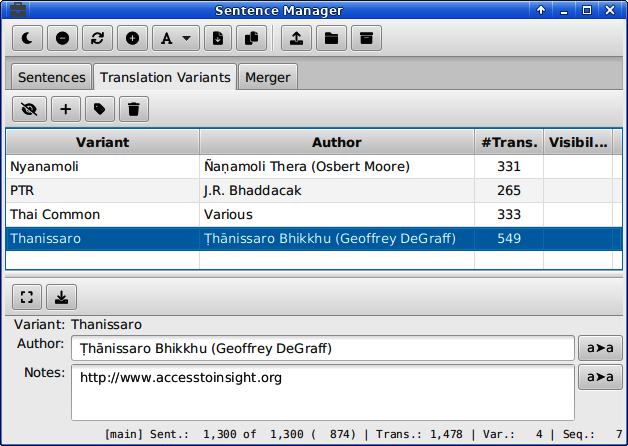
\includegraphics[width=0.9\linewidth]{images/sentmanager-variants.png}\\
\caption{Translation Variants in Sentence Manager}
\label{fig:sentmanager-variants}
\end{figure}

If you want to delete all translations under a variant name, you can delete that variant by {\faSix \symbol{"F1F8}} button. This causes all sentences containing the variant to get updated. Be careful, you cannot undo this action and a lot of data may be lost. Make sure you have a backup, and you are sober enough at the moment. If you just want to rename the variant, use {\faSix \symbol{"F02B}} button instead. I leave other minor things in this tab to the users to find out by themselves.

\section{Merger}

The last tab of the Manager is the sentence directory merger (Figure \ref{fig:sentmanager-merger}). It is really useful in practice. Without this tool, you have to do many of tedious works manually. The tool has a simple purpose: to merge two directories into one with simple steps.

\begin{figure}[!hbt]
\centering
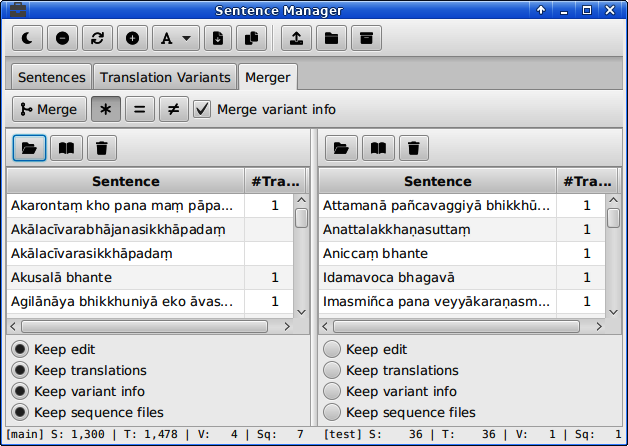
\includegraphics[width=0.9\linewidth]{images/sentmanager-merger.png}\\
\caption{Merger in Sentence Manager}
\label{fig:sentmanager-merger}
\end{figure}

First, you have to create more than one sentence directories. You can test this by selecting a sequence and saving it in a new directory. Do it again with another sequence. Then you load these two directories into the Merger, left and right.

Now you have to think whether you should merge variant information or not. And think further, if a crash occurs (when two directories contain the same sentence), which one you want to keep its data. The options to set lie in the lower part.

Once you finish the settings, hit {\faSix \symbol{"F387}} Merge button. It will ask you for the output directory. You should create a new one or select an empty one. When done, you will see the magic.

To understand all the things we have talked about here, as well as unmentioned parts, you have to roll the sleeves up and get your hand dirty. I keep this section short, albeit the tool's operations are really complex, because the only way to learn the tool effectively is by playing with it.

